\section{Results}
\label{sec:results}

\begin{figure}
	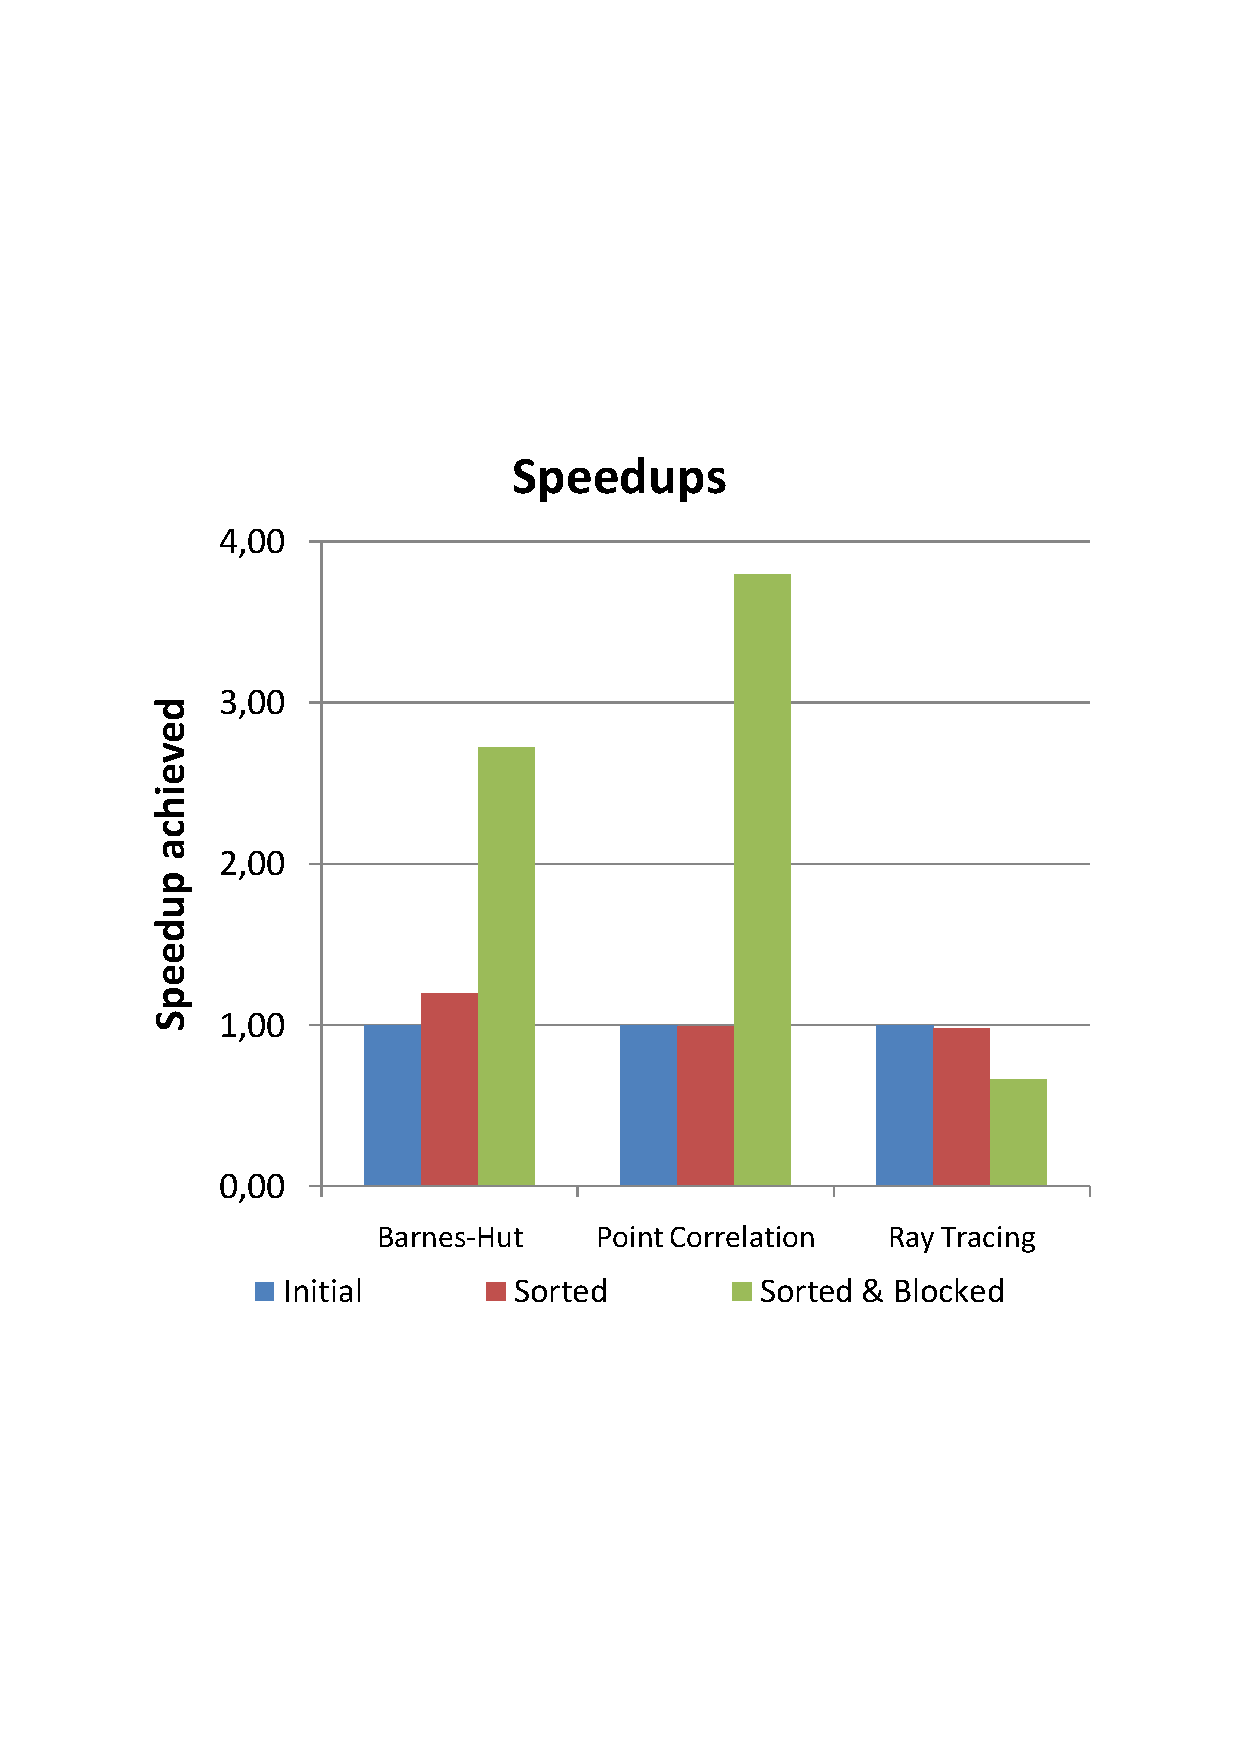
\includegraphics[width=\columnwidth]{speedups.pdf}
	\caption{Speedups attained using Sorting and Point Blocking for each of the three implemented examples.}
	\label{fig:speedups}
\end{figure}

% BH	2.7
% PC	3.82
% RT	0.7

\Cref{fig:speedups} shows the improvements in execution time obtained with the optimizations described in this document when applied to the three implemented examples. PC got the largest speedup of 3.79 from using Sorting and Point Blocking, followed by BH with a speedup of 2.7, while RT did not achieve better execution times. To notice that the PC algorithm did not benefit at all from using only Sorting. This can be easily explained by the input generator, which was copied from the BH original implementation in Galois, and may not be suitable for the PC problem. The lack of speedup in the RT example can be easily explained by the increased complexity behind managing the blocks.

% BH
%	L1	62%
%	L2	8%
%	L3	4%

% PC
%	L1	68%
%	L2	2%
%	L3	3%

% RT
%	L1	82%
%	L2	54%
%	L3	63%

\begin{figure}
	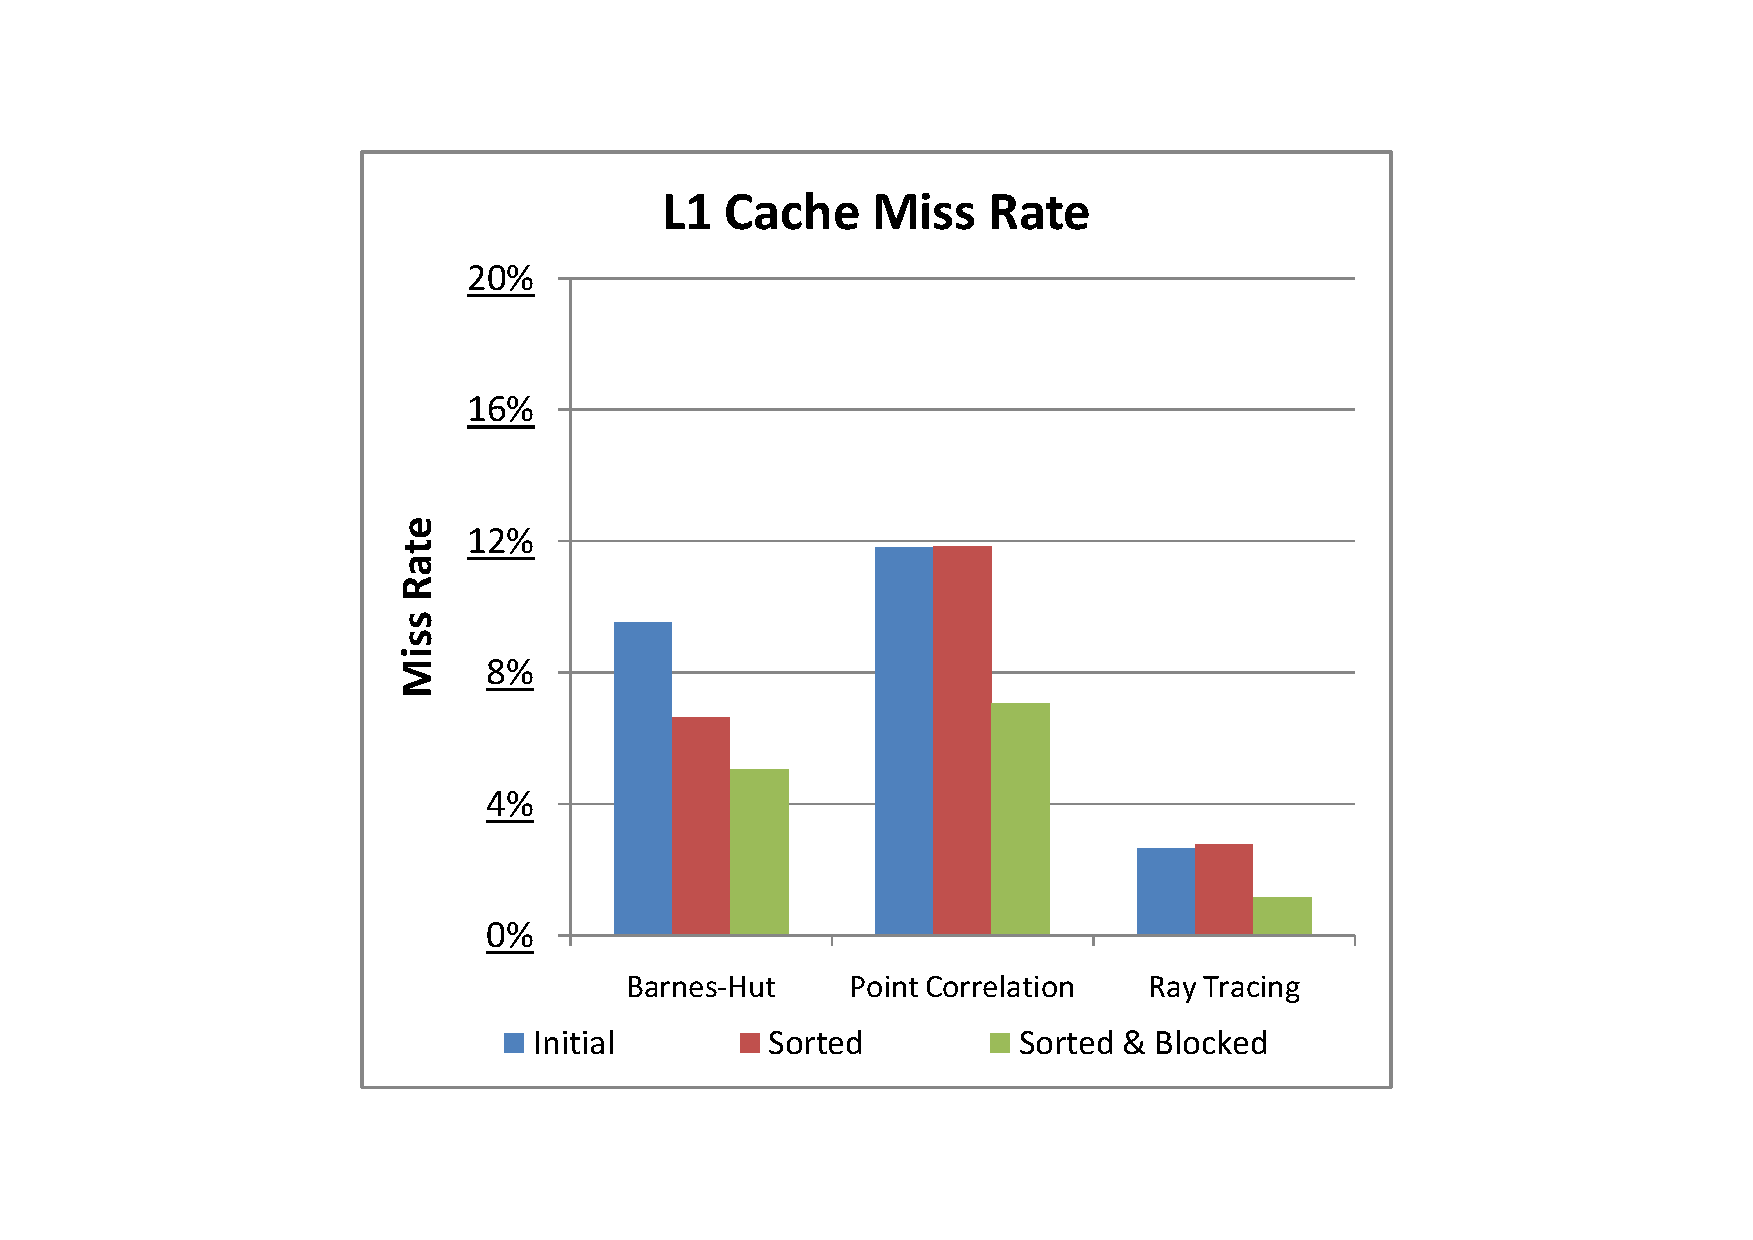
\includegraphics[width=\columnwidth]{missrate-l1.pdf}
	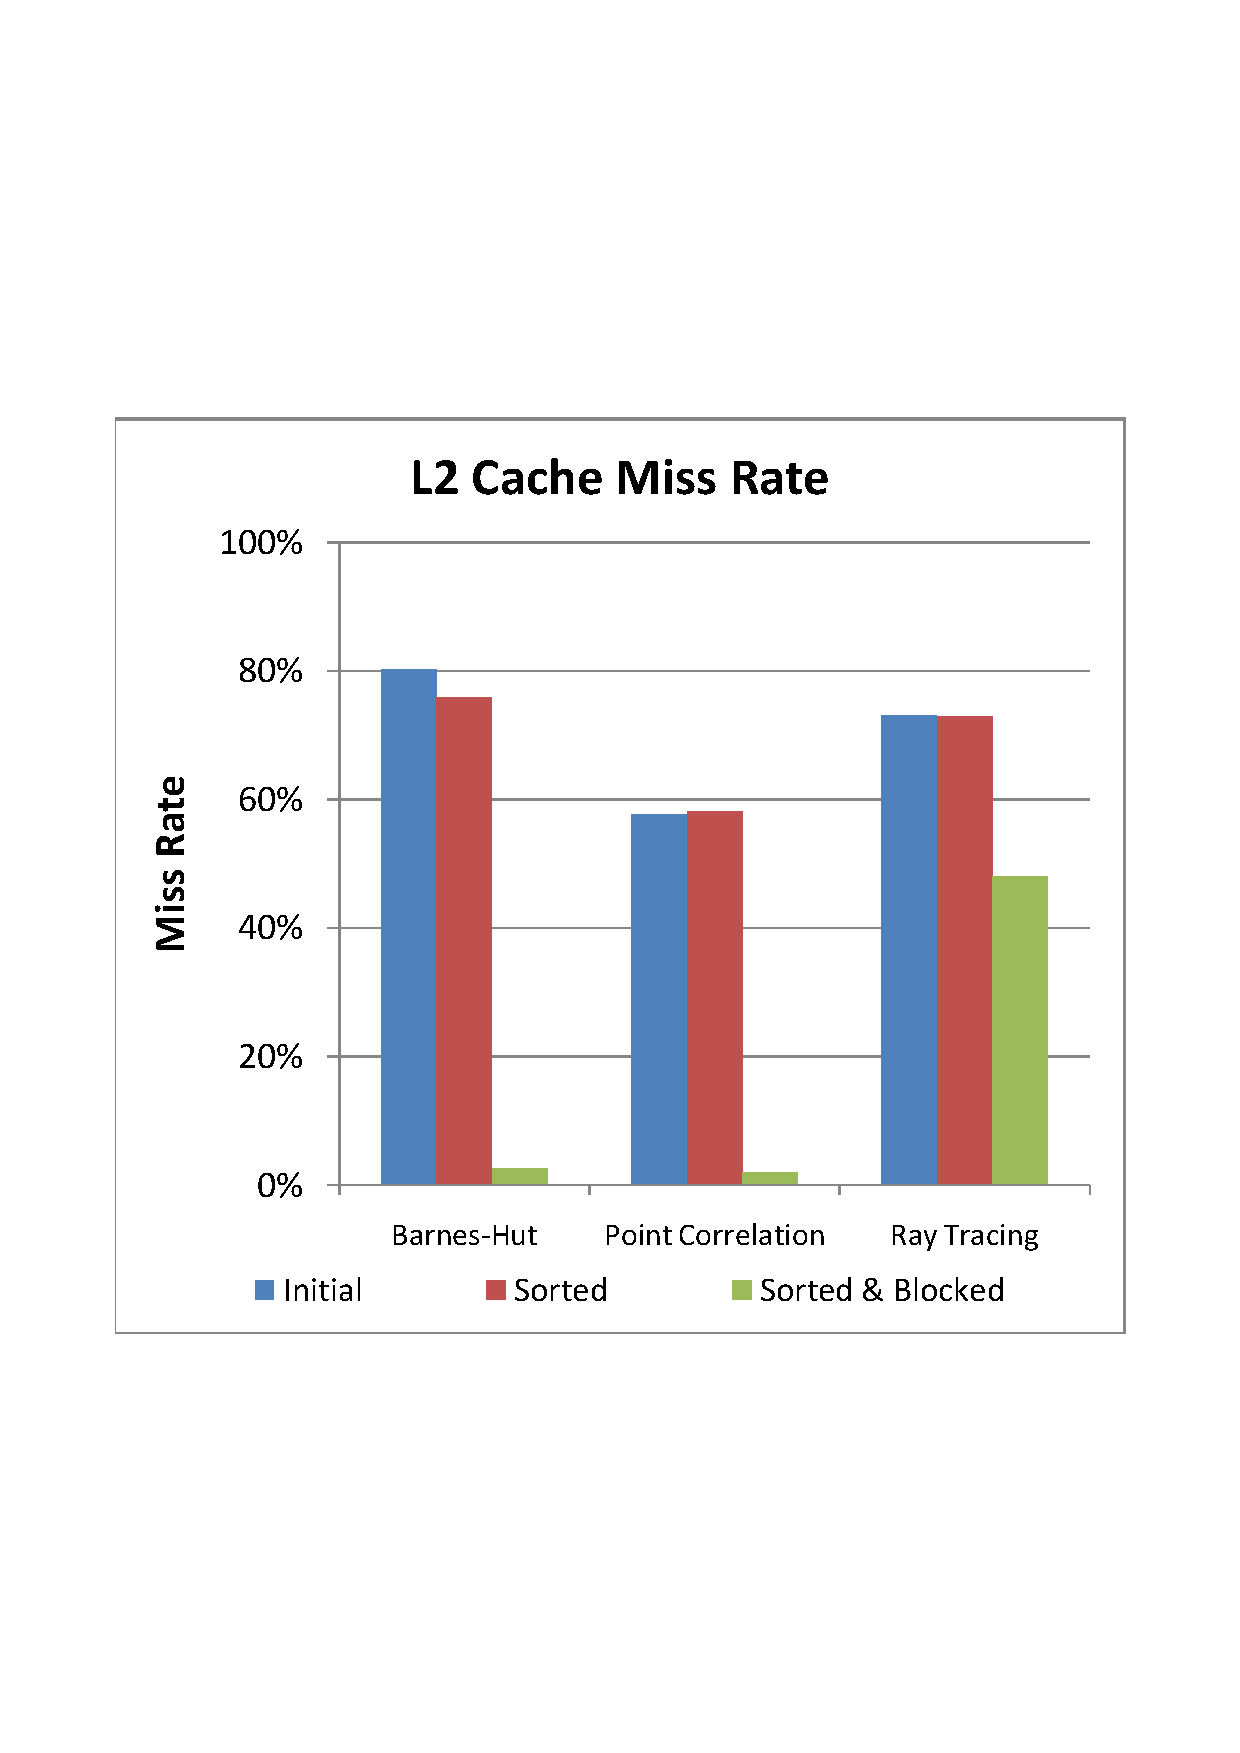
\includegraphics[width=\columnwidth]{missrate-l2.pdf}
	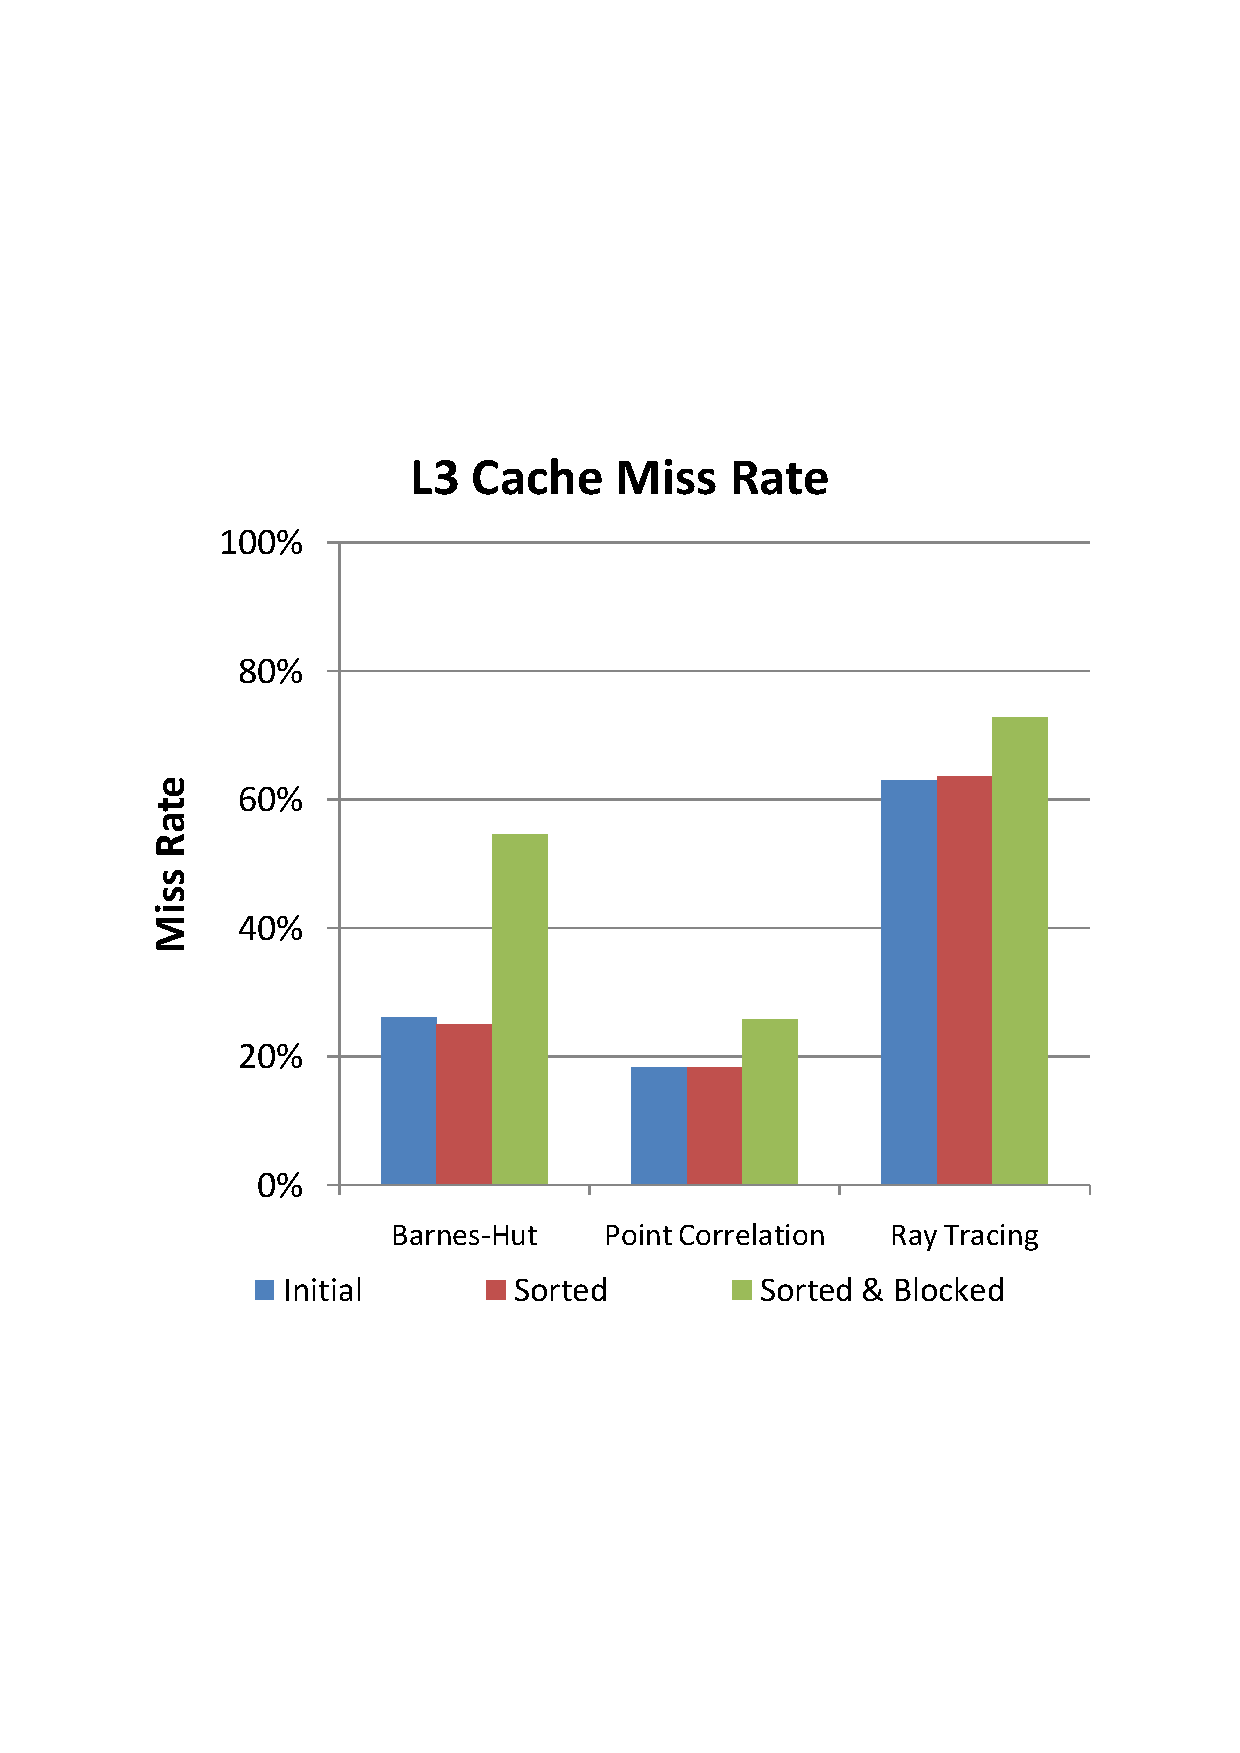
\includegraphics[width=\columnwidth]{missrate-l3.pdf}
	\caption{Cache miss rates in each level for the base version and using the two optimizations for each of the described examples.}
	\label{fig:misses}
\end{figure}

Despite the RT not achieving a better execution time, \cref{fig:misses} shows that it benefited from the described optimizations in cache levels 1 and 2. The reported speedups can also be justified by a significant decrease in cache miss rates in the same two levels due to the increase of locality. The figure shows decreases around 5\% in the first level of cache for both BH and PC, but only a neglectable 1\% for RT. The best improvements are shown in L2, where BH decreased the miss rate by almost 80\%, PC decreased by more than 50\% and RT decreased the miss rate by 25\%. In the last level of cache, no improvements are shown for any of the examples.
